% The mandatory-group mirror of `keyval_optionals.tex`: every command here is
% curated `{"kind": "req", "content": "keyval"}`, so the formatter may split its
% brace argument at a comma the author *glued* — materializing a space token TeX
% sees. Each key list is authored on one long line so the split actually fires.
\documentclass[a4paper,11pt]{article}
\usepackage{geometry,graphicx,tikz,listings,pgfplots,siunitx,enumitem,caption,hyperref}
\geometry{margin=2cm,heightrounded,includeheadfoot,footskip=1cm,headsep=5mm}
\hypersetup{colorlinks=true,linkcolor=blue,citecolor=green,urlcolor=magenta,bookmarks=true}
\pgfplotsset{compat=1.18,width=6cm,height=4cm,tick label style={font=\small}}
\pgfkeys{/tikz/.cd,sample color/.initial=black,sample size/.initial=1pt,sample width/.initial=2pt}
\tikzset{boxed/.style={draw,thick,rounded corners,inner sep=2pt,fill=yellow!20},every node/.append style={align=center}}
\lstset{basicstyle=\ttfamily,numbers=left,numberstyle=\tiny,frame=single,breaklines=true}
\sisetup{per-mode=symbol,round-mode=places,round-precision=3,group-separator={,}}
\setlist[itemize]{leftmargin=*,noitemsep,topsep=0pt,partopsep=0pt,parsep=0pt,itemsep=2pt}
\captionsetup[figure]{font=small,labelfont=bf,labelsep=period,justification=centering}
\begin{document}
\section{S}
Text with \href{https://example.com}{a link} and \SI{1.23456}{\metre\per\second}.
\begin{itemize}
  \item first
  \item second
\end{itemize}
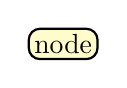
\begin{tikzpicture}
  \node[boxed] at (0,0) {node};
\end{tikzpicture}\par
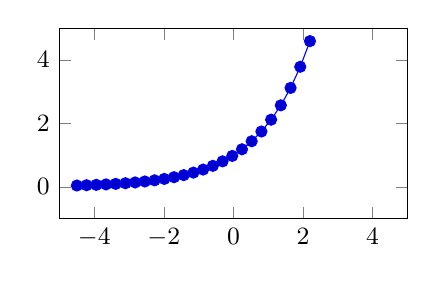
\begin{tikzpicture}
  \begin{axis}[xmin=-5,xmax=5,ymin=-1,ymax=5]
    \addplot expression[domain=-4.5:2.2]{2^x};
  \end{axis}
\end{tikzpicture}\par
\begin{figure}[htb]
  \includegraphics[width=3cm]{example-image}
  \caption{Full caption}
\end{figure}
\begin{lstlisting}
x = 1
\end{lstlisting}
\end{document}
